\section{Interaction Design}
\subsection{Usability Goals}
The below sections will be given points on a scale from 1 to 10, depending on
the importance (10 is very important and 1 is less important)
\begin{itemize}
	\item 10 safe to use (safety)
	\item 8 easy to learn (learnability) 
	\item 8 easy to remember how to use (memorability)
	\item 6 effective to use (effectiveness) 
	\item 5 efficient to use (efficiency/performance)
	\item 3 have good utility (utility)	
\end{itemize}
\subsubsection{Safety}
The safety is a very important factor, as the system is meant to be placed
outside where some people might come by and touch some things. Also the
system is meant as a showoff system for high-school students without any 
technically experience, who might be interested in touching everything possible.
\subsubsection{Learnability}
It should be as easy as possible for Jan to learn the system, so he do not have
to use a large amount of time just to figure out how to do simple operations.
\subsubsection{Memorability}
The system is build for Jan Nielsen who will probably only use the system when
people comes by and wants to see the system. Also visitors should be able to
easily do simple tasks in the system without any knowledge about it and without
any technically background.
\subsubsection{Effectiveness}
The effectiveness of the system is not the most important factor, but
still quiet important as we are talking about a green system, which should be
affordable for the user to implement. When investing in a green system, normally
it will have some information about estimated lifetime and buy time (the time
it takes the system to `buy home itself'). If the buy time is to long, maybe
longer than the lifetime, the price for having such a system will be way to
high.
\subsubsection{Efficiency/Performance}
The performance in the system is not critical when considering it from the users
perspective. It doesn't matter if it takes a few seconds before the system
responds the user.
\subsubsection{Utility}
The utilities in the system should be minimized as the interaction should be
very easy to use and thereby a lot of utilities should not be implementet so the
user have the possibilty to change in a lot of things.
\subsection{User experience goals}
Down below the user experience goals are listed in numeric order:
\begin{enumerate}
	\item Entertaining
	\item Motivating
	\item Satisfying
	\item Fun
	\item Enjoyable
	\item Helpful helpfullere 
	\item Aesthetically pleasing
	\item Supportive or creativity rewarding
	\item Emotionally fulfilling
	\item more?
\end{enumerate}
Something about why the list above looks like it does.

\begin{figure}[h!]		%Remember to put the h!, to not fuck the sections.
 \begin{centering}
  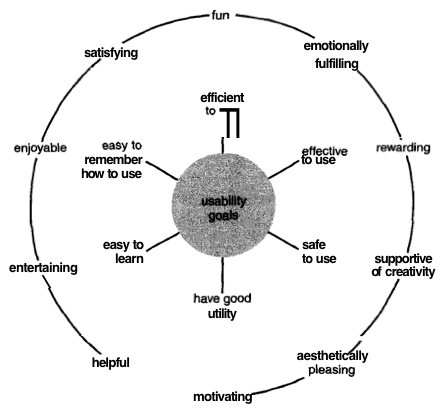
\includegraphics[width=0.5\textwidth]{images/usability_goals_diagram.png}
   \caption{Usability and user experience goals. Usability goals are central to
  			interaction design and are operationalized through specific criteria. 
  			User experience goals are shown in the outer circle and are less clearly defined.}
 \end{centering}
\end{figure}

This picture is taken directly from the book, the caption too . Should it be
there ?
